\documentclass[11pt,a4paper]{article}

% ---- encoding & language ----
\usepackage[utf8]{inputenc}
\usepackage[T1]{fontenc}
\usepackage[shorthands=off,turkish]{babel}  % shorthands off: Turkish '=' shorthand breaks keyval (\includegraphics, tcolorbox)

% ---- fonts (Helvetica-like) ----
\usepackage{helvet}
\renewcommand{\familydefault}{\sfdefault}

% ---- layout ----
\usepackage[a4paper,margin=2.3cm]{geometry}
\usepackage{graphicx}
\usepackage{xcolor}
\usepackage[most]{tcolorbox}
\usepackage{booktabs}
\usepackage{amsmath,amssymb}
\usepackage{caption}
\usepackage{float}
\usepackage{enumitem}
\usepackage[hidelinks]{hyperref}

\captionsetup{font=small,labelfont=bf}
\setlength{\parskip}{0.55em}
\setlength{\parindent}{0pt}

% ---- palette ----
\definecolor{cblue}{HTML}{185FA5}
\definecolor{cbluebg}{HTML}{E6F1FB}
\definecolor{cgreen}{HTML}{3B6D11}
\definecolor{cgreenbg}{HTML}{EAF3DE}
\definecolor{camber}{HTML}{BA7517}
\definecolor{camberbg}{HTML}{FAEEDA}
\definecolor{cred}{HTML}{A32D2D}
\definecolor{credbg}{HTML}{FCEBEB}
\definecolor{cgray}{HTML}{444441}
\definecolor{cgraybg}{HTML}{F1EFE8}

% ---- boxes ----
\newtcolorbox{ozet}[1][Özet]{colback=cbluebg,colframe=cblue,fonttitle=\bfseries,
  title={#1},boxrule=0.8pt,arc=2pt,left=6pt,right=6pt,top=4pt,bottom=4pt}
\newtcolorbox{bulgu}[1][Ana bulgu]{colback=cbluebg,colframe=cblue,fonttitle=\bfseries,
  title={#1},boxrule=0.8pt,arc=2pt,left=6pt,right=6pt,top=4pt,bottom=4pt}
\newtcolorbox{yontem}[1][Yöntem]{colback=cgreenbg,colframe=cgreen,fonttitle=\bfseries,
  title={#1},boxrule=0.8pt,arc=2pt,left=6pt,right=6pt,top=4pt,bottom=4pt}
\newtcolorbox{uyari}[1][Sınırlama]{colback=camberbg,colframe=camber,fonttitle=\bfseries,
  title={#1},boxrule=0.8pt,arc=2pt,left=6pt,right=6pt,top=4pt,bottom=4pt}
\newtcolorbox{kritik}[1][Kritik]{colback=credbg,colframe=cred,fonttitle=\bfseries,
  title={#1},boxrule=0.8pt,arc=2pt,left=6pt,right=6pt,top=4pt,bottom=4pt}

\newcommand{\msp}{I_{\mathrm{sp}}}
\newcommand{\dmatch}{\textcolor{cgreen}{\textbf{Eşleşiyor}}}
\newcommand{\ddiff}{\textcolor{cred}{\textbf{Farklı}}}
\newcommand{\dpart}{\textcolor{camber}{\textbf{Kısmî}}}
\newcommand{\dunspec}{\textcolor{camber}{\textbf{Belirtilmemiş}}}

\begin{document}

% ===================== TITLE =====================
\begin{center}
{\LARGE\bfseries SNCP--PPO ile Kalabalıkta İnsan-Merkezli Navigasyon}\\[4pt]
{\large Ao vd.\ (2026) Reprodüksiyonu: v18\,$\rightarrow$\,v27 İlerleme Durum Raporu}\\[10pt]
{\normalsize Orkun Koray Güngör}\\[2pt]
{\small 17 Haziran 2026 — Güncel durum raporu}
\end{center}
\vspace{4pt}
\hrule
\vspace{8pt}

\begin{ozet}
Bu çalışma, Ao vd.\ (2026, \textit{Int.\ J.\ Social Robotics}) makalesindeki SNCP--PPO
mimarisini (Yapısal Nöral Devre Politikası + PPO) yeniden üretmeyi amaçlar. Makale, kalabalık
``challenging'' senaryosunda \%94 başarı / \%4 çarpışma bildirir. Uzun bir teşhis dizisinden
(v18--v26) sonra, \textbf{v26} bütçe/geometri/konfor düzeltmeleriyle paper rejimini sadık biçimde
kurar: \emph{zaman aşımı her yoğunlukta sıfırlanır} ve başarısızlık tamamen \emph{çarpışmaya} indirgenir.
Yerel çok-tohumlu (multi-seed) dürüst değerlendirme, N=10 yayada \textbf{\%61.6} (\%95 GA [55.6, 67.6])
başarı verir; makalenin \%94'üne kıyasla iki ayrı açık kalır: (a) eğitilen yoğunlukta dahi 32 puanlık
\emph{temel} açık, (b) yüksek yoğunlukta düşüş. Ayrıca, eğitim-içi ``best holdout'' ölçütünün
\textbf{seçim-saplı} (selection-biased) olduğu kanıtlanır; sürüm kıyasları bundan böyle çok-tohumlu
yapılmalıdır. Bir sonraki tek-değişkenli deney olan \textbf{v27}, makalenin Denklem~11 ön-MLP
gömmesini ekler ve yarın eğitilecektir.
\end{ozet}

% ===================== 1. GİRİŞ =====================
\section{Giriş ve Problem Tanımı}

Kalabalık ortamlarda hareket planlama, bir mobil robotun hedefe \emph{hızlı} ulaşması ile çevredeki
insanların \emph{konforunu} koruması arasındaki çok-amaçlı bir gerilimdir. Referans aldığımız çalışma
(Ao vd., 2026), bu problemi \emph{Yapısal Nöral Devre Politikası} (Structured Neural Circuit Policy,
SNCP) ile çözer: insan-robot etkileşimini uzay-zamansal bir grafa dönüştürür, üç ayrı NCP kodlayıcı ile
(robot düğümü, zamansal kenar, uzaysal kenar) işler, dikkat (attention) havuzlamasıyla kalabalığı tek bir
vektöre indirger ve PPO ile uçtan uca eğitir. Robot eylemi $a_t=(\omega_t, v_t)$ (açısal ve doğrusal hız)
bir tekerlekli (unicycle) modeldir ve gerçek bir TurtleBot~2 üzerinde konuşlandırılır.

Projemizin amacı bu sonucu \emph{kendi uygulamamızda} yeniden üretmektir. Mimari, ödül fonksiyonu, yaya
modeli (ORCA) ve PPO hattı makaleyle eşleşmesine rağmen, uzun süre \%94 başarıya ulaşamadık. Bu rapor,
o açığın nereden geldiğini sistematik biçimde nasıl daralttığımızı, v26'nın \emph{dürüst} (önyargısız)
performansını ve bir sonraki adımı (v27) bilimsel ayrıntısıyla belgeler.

\begin{kritik}[Anti-abartı kültürü]
Bu raporun ana ilkesi: her sayıyı yer-gerçeğine (kod + makale PDF'i + ham deney çıktısı) karşı
\emph{denetlemek}. Aşağıda gösterileceği gibi, eğitim-içi ``en iyi'' (best) sayıları tek başına
güvenilmezdir; bu rapordaki tüm v26 başarı sayıları bağımsız çok-tohumlu değerlendirmeden gelir.
\end{kritik}

% ===================== 2. YÖNTEM =====================
\section{Yöntem ve Mimari}

\begin{yontem}[Eğitim ve değerlendirme rejimi (v26 paper rejimi)]
\textbf{Senaryo:} \texttt{paper\_challenging} (dağınık yayalar, $15\times15$ m arena, algı yarıçapı 6 m).
\textbf{Geçiş:} robot $(0,-4)\!\rightarrow\!(0,4)$, yani 8 m (makale §5.3.2). \textbf{Robot hızı:} 1.0 m/s
(unicycle). \textbf{Yayalar:} ORCA, hız paritesi 1.0 m/s, görünmez-robot rejimi. \textbf{Bütçe:}
challenging 50 s, standard 12.5 s (per-senaryo, ortamdan türetilir). \textbf{Çarpışma eşiği:}
$d_{\mathrm{col}}=0.3$ m. \textbf{Konfor katsayısı:} 2.0. \textbf{Öğrenme oranı:} $10^{-4}$.
\textbf{Bütçe:} 2.5\,M adım, 16 paralel ortam $\times$ 128 ufuk, sıfırdan (IL ısıtması yok).
\end{yontem}

Politika ağı (Şekil~\ref{fig:arch}), makaledeki anlamsal bölümlemeyi izler. Robot düğümü bir MLP ile
128 boyuta gömülür (Denklem~14). Zamansal ve uzaysal kenarlar birer Sıvı Zaman-Sabitli ağ (Liquid
Time-Constant, LTC; sparse AutoNCP kablolaması) ile işlenir. Dikkat havuzlaması, her yayanın uzaysal
özniteliğini robot/zaman anahtarına göre ağırlıklandırır:
\begin{equation}
\alpha^t=\mathrm{softmax}\!\left(\frac{n}{\sqrt{d_k}}\,Q^t (K^t)^{\!\top}\right),\qquad
u^t_{\mathrm{att}}=(M^t_{r\text{-}h})^{\!\top}\alpha^t , \tag{Eq.\ 13}
\end{equation}
burada $d_k=64$ ve $n$ yaya sayısıdır. Füzyon düğümü NCP'si robot (128) + zaman (256) + dikkat (256)
$=640$ boyutu birleştirir; actor--critic başı $(\omega,v)$ ve değeri üretir (Denklem~16).

\paragraph{Ödül fonksiyonu (makale Denklem 17--20).} Çok amaçlı ödül üç terimden oluşur,
$r_{\mathrm{total}}^t = r_g^t + r_c^t + r_s^t$:
\begin{align}
r_g^t &= \begin{cases} 20, & \lVert p^t-p_g\rVert < p'_{\mathrm{robot}}\\[2pt]
2\big(\lVert p^{t-1}-p_g\rVert - \lVert p^t-p_g\rVert\big), & \text{aksi halde} \end{cases}
\tag{Eq.\ 18}\\[4pt]
r_c^t &= \begin{cases} -20, & d_{\min} < d_{\mathrm{col}}\\ 0, & \text{aksi halde} \end{cases}
\qquad\qquad r_s^t = -2\,\msp . \tag{Eq.\ 19--20}
\end{align}
Sosyal baskı indeksi $\msp$ (konfor) makalenin Denklem~5--7'sinde, komşu yayaların ters-mesafe
ağırlıklı \emph{normalize} ortalaması olarak tanımlanır ($\msp\in[0,1]$). v26'da bu terim, kodumuzdaki
eski (normalize edilmemiş + kırpılmış) hatadan, makaledeki normalize forma düzeltilmiştir.

\begin{figure}[H]
\centering
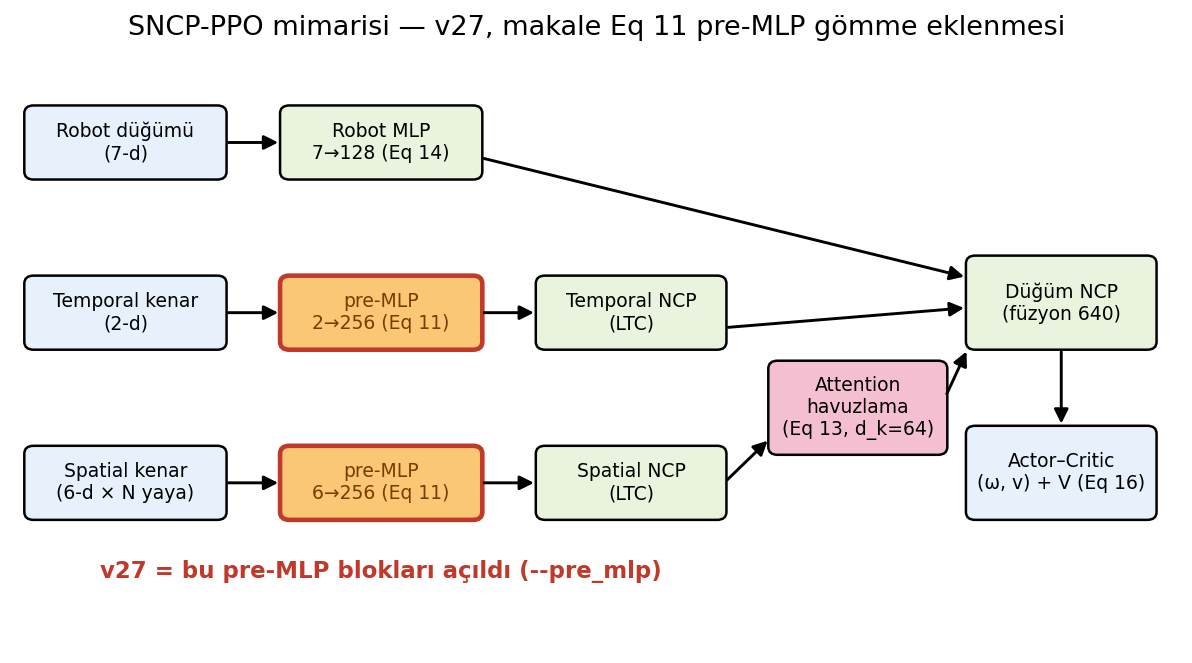
\includegraphics[width=0.97\textwidth]{figures/fig_arch.png}
\caption{SNCP--PPO politika mimarisi. v27, makalenin Denklem~11 ön-MLP gömmesini (turuncu bloklar)
açar: ham kenar girdisi NCP'ye girmeden önce bir MLP ile 256 boyuta yükseltilir. v26 (varsayılan)
ham 2/6 boyutlu sinyali doğrudan NCP'ye verir — Denklem~11'den gerçek bir sapma.}
\label{fig:arch}
\end{figure}

\paragraph{Değerlendirme protokolü.} Politika belirlenimci (deterministic) modda çalıştırılır
(eylem $=\mu$). Yoğunluk taraması N=5/10/15/20 yayada; her yoğunlukta 50 bölüm. Sürüm kıyasları için
\emph{çok-tohumlu} (5 tohum $\times$ 50 bölüm $=250$ bölüm/yoğunluk) havuzlanmış oran ve \%95 güven
aralığı raporlanır.

% ===================== 3. MAKALE KARŞILAŞTIRMASI =====================
\section{Makale ile Birebir Karşılaştırma}

Bu bölüm, mevcut uygulamamızdaki (v26/v27) her değişkeni makaledeki karşılığıyla karşılaştırır ve
makalede \emph{belirtilmeyen} değişkenleri açıkça işaretler. Kategori bazında özet
Şekil~\ref{fig:compare}'de verilmiştir: 29 değişken eşleşir, 4'ü farklı/kısmîdir (çoğu v27'de
ele alınıyor) ve \textbf{12 değişken makalede hiç belirtilmemiştir} -- bunlar bizim mühendislik
seçimlerimizdir.

\begin{figure}[H]
\centering
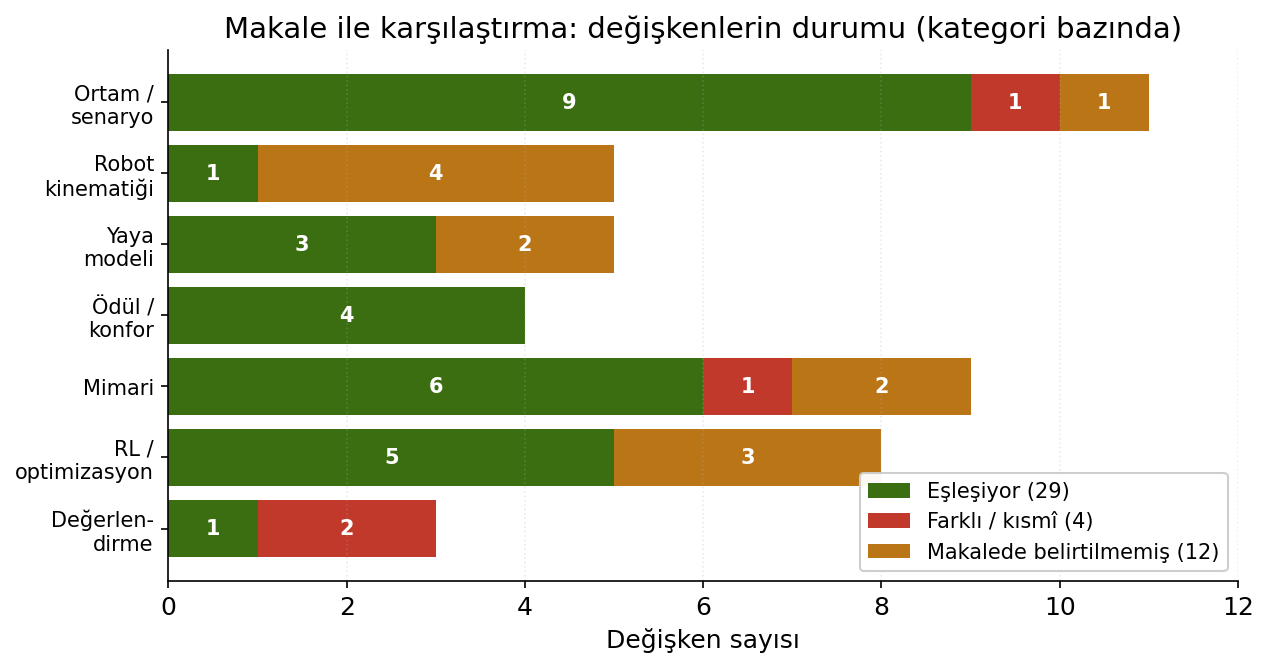
\includegraphics[width=0.92\textwidth]{figures/fig_compare.png}
\caption{Makale ile karşılaştırmanın kategori bazında özeti. Yeşil: eşleşiyor; kırmızı: farklı/kısmî;
turuncu: makalede belirtilmemiş (mühendislik seçimimiz). Belirtilmeyen 12 değişkenin çoğu mimari
kablolaması, eylem aralıkları ve eğitim/değerlendirme bütçesidir.}
\label{fig:compare}
\end{figure}

\subsection{Makalenin bildirdiği hedef metrikler}

Karşılaştırmanın çapası, makalenin SNCP--PPO için bildirdiği sonuçlardır (Tablo~\ref{tab:papermetrics}).
Bizim dürüst N=10 sonucumuz (\%61.6) bu challenging hedefin (\%94) altındadır; standart senaryo henüz
ayrıca raporlanmamıştır.

\begin{table}[H]
\centering\small
\caption{Makalenin SNCP--PPO için bildirdiği metrikler (Tablo 2--3).}
\begin{tabular}{@{}lccccc@{}}
\toprule
\textbf{Senaryo} & \textbf{Başarı} & \textbf{Çarpışma} & \textbf{Zaman aşımı} & \textbf{Konfor} & \textbf{Nav-süre} \\
\midrule
Standard (5 yaya)      & 0.995 & 0.005 & 0.000 & 0.997 & 10.39 s \\
Challenging (10--20)   & 0.94  & 0.04  & 0.02  & 0.962 & 15.92 s \\
\bottomrule
\end{tabular}
\label{tab:papermetrics}
\end{table}

\subsection{Ortam ve senaryo değişkenleri}

\begin{table}[H]
\centering\small
\begin{tabular}{@{}p{3.2cm}p{4.0cm}p{4.4cm}l@{}}
\toprule
\textbf{Değişken} & \textbf{Makale} & \textbf{Bizde (v26)} & \textbf{Durum} \\
\midrule
Standart arena & $10\times10$ m & $10\times10$ m & \dmatch \\
Challenging arena & $15\times15$ m & $15\times15$ m & \dmatch \\
Standart algı menzili & 4 m (\S5.1.2)$^{*}$ & 4 m & \dmatch \\
Challenging algı menzili & 6 m & 6 m & \dmatch \\
Standart yaya sayısı & 5 & 5 & \dmatch \\
Challenging yaya sayısı & 10--20 & eğitim sabit 10; eval 5--20 & \dpart \\
Robot geçişi & $(0,-4)\!\rightarrow\!(0,4)=8$ m & 8 m & \dmatch \\
Çarpışma eşiği $d_{\mathrm{col}}$ & 0.3 m & 0.3 m & \dmatch \\
Robot hızı (sim) & 1.0 m/s & 1.0 m/s & \dmatch \\
Zaman adımı & 0.25 s & 0.25 s & \dmatch \\
Süre bütçesi $t_{\lim}$ & 12.5 s (Tablo 1, standart) & std 12.5 / chal 50 s & \dunspec \\
\bottomrule
\end{tabular}
\par{\scriptsize $^{*}$Tablo 1 ``observation range 3 m'' der; \S5.1.2 ise 4/6 m verir -- makale-içi çelişki.
Challenging bütçesi makalede ayrıca verilmez; Tablo 3'teki 15.92 s nav-süresi 12.5 s'i imkânsız kılar,
biz 50 s aldık.}
\end{table}

\subsection{Robot kinematiği ve yaya modeli}

\begin{table}[H]
\centering\small
\begin{tabular}{@{}p{3.2cm}p{4.0cm}p{4.4cm}l@{}}
\toprule
\textbf{Değişken} & \textbf{Makale} & \textbf{Bizde} & \textbf{Durum} \\
\midrule
Eylem uzayı & $a_t=(\omega,v)$ unicycle (Eq 16) & $(\omega,v)$ unicycle & \dmatch \\
Doğrusal hız aralığı $v$ & belirtilmemiş (sim)$^{\dagger}$ & $[0,\ 1.0]$ m/s & \dunspec \\
Açısal hız sınırı $\omega_{\max}$ & belirtilmemiş & 1.8 rad/s & \dunspec \\
Geri hareket (reverse) & belirtilmemiş & yok ($v\geq0$) & \dunspec \\
Maks ivme (sim) & belirtilmemiş$^{\ddagger}$ & modellenmez & \dunspec \\
Yaya modeli & ORCA & ORCA & \dmatch \\
Yaya hızı & $\sim$1.0 m/s & 1.0 m/s (parite) & \dmatch \\
Görünmez robot & evet & evet & \dmatch \\
ORCA parametreleri & belirtilmemiş & varsayılan seçimimiz & \dunspec \\
Yaya hedef davranışı & Fig 7: statik (respawn yok) & varınca durur & \dunspec \\
\bottomrule
\end{tabular}
\par{\scriptsize $^{\dagger}$Gerçek robot (\S5.3.5): $v_{\max}$ 0.7 m/s, çap 0.35 m, 10 Hz planlama.
$^{\ddagger}$Gerçek robot $a_{\max}$ 1.0 m/s$^2$; sim için verilmez.}
\end{table}

\subsection{Ödül, konfor ve mimari}

\begin{table}[H]
\centering\small
\begin{tabular}{@{}p{3.2cm}p{4.0cm}p{4.4cm}l@{}}
\toprule
\textbf{Değişken} & \textbf{Makale} & \textbf{Bizde} & \textbf{Durum} \\
\midrule
$r_g$ (Eq 18) & 20 / $2\cdot\Delta d$ & 20 / $2\cdot\Delta d$ & \dmatch \\
$r_c$ (Eq 19) & $-20$ & $-20$ & \dmatch \\
$r_s$ (Eq 20) & $-2\,\msp$ & $-2\,\msp$ (konfor 2.0) & \dmatch \\
$\msp$ (Eq 5--7) & normalize ağırlıklı ort. & normalize (v26'da düzeltildi) & \dmatch \\
Robot düğüm gömme & 128 & 128 & \dmatch \\
Zaman kenarı gömme & 256 & 256 (v27 ön-MLP) & \dmatch \\
Uzay kenarı gömme & belirtilmemiş & 256 (seçimimiz) & \dunspec \\
Dikkat boyutu $d_k$ & 64 & 64 & \dmatch \\
Dikkat ölçeği (Eq 13) & $n/\sqrt{d_k}$ ($n$ var) & $1/\sqrt{d_k}$ ($n$ yok) & \ddiff \\
Eq 11 ön-MLP & var (ham$\rightarrow$MLP$\rightarrow$NCP) & v27 ekler; v26 atlar & \dmatch \\
NCP tipi & NCP (LTC) & LTC (\texttt{ncps}) & \dmatch \\
NCP kablolaması & belirtilmemiş & AutoNCP (units/sparsity) & \dunspec \\
Füzyon & robot+zaman+dikkat$\rightarrow$NCP & 640$\rightarrow$NCP & \dmatch \\
\bottomrule
\end{tabular}
\par{\scriptsize Dikkat $n$ faktörü (Eq 13) ve Eq 11 ön-MLP makaleye sadıktır; v27 ön-MLP'yi açar,
$n$-ölçeklemesi ayrı bir tek-değişkenli deneye ertelenmiştir.}
\end{table}

\subsection{RL/optimizasyon ve değerlendirme}

\begin{table}[H]
\centering\small
\begin{tabular}{@{}p{3.2cm}p{4.0cm}p{4.4cm}l@{}}
\toprule
\textbf{Değişken} & \textbf{Makale} & \textbf{Bizde} & \textbf{Durum} \\
\midrule
Algoritma & PPO & PPO & \dmatch \\
PPO clip $\epsilon$ & 0.2 & 0.2 & \dmatch \\
İndirim $\gamma$ & 0.99 & 0.99 & \dmatch \\
Öğrenme oranı & $10^{-4}$ & $10^{-4}$ & \dmatch \\
Replay buffer (Alg 1) & var & var (vektörize) & \dmatch \\
Toplam eğitim bütçesi & belirtilmemiş & 2.5\,M adım & \dunspec \\
Paralel ortam / batch & belirtilmemiş & 16 ortam $\times$ 128 & \dunspec \\
Müfredat (curriculum) & belirtilmemiş & easy$\rightarrow$sabit-N & \dunspec \\
Test örneği sayısı & 500/yoğunluk ($\times$11 grup) & 50/yoğunluk & \ddiff \\
Metrikler & Succ/Coll/TO/Konfor/Nav & aynı + $\msp$ & \dmatch \\
Çoklu-tohum & tek model, 500 test & 5 tohum $\times$ 50 & \ddiff \\
\bottomrule
\end{tabular}
\end{table}

\begin{uyari}[Makalede belirtilmeyen 12 değişken (bizim seçimlerimiz)]
\textbf{Mimari:} (1) uzay-kenarı gömme boyutu, (2) NCP kablolaması (units/sparsity/motor).
\textbf{Eylem:} (3) doğrusal hız aralığı, (4) $\omega_{\max}$, (5) geri hareket, (6) sim ivme/planlama frekansı.
\textbf{Yaya:} (7) ORCA parametreleri (time horizon, komşu mesafesi), (8) hedefe varınca davranış (respawn/durma).
\textbf{Eğitim/değerlendirme:} (9) challenging zaman bütçesi (sadece standart 12.5 s verilir), (10) toplam
eğitim bütçesi, (11) paralel ortam/batch, (12) curriculum.
\textbf{Makale-içi çelişkiler:} algı menzili (Tablo 1: 3 m vs \S5.1.2: 4/6 m); $t_{\lim}$ (Tablo 1: 12.5 s vs
Tablo 3 challenging nav-süresi 15.92 s). Bu belirsizlikler, reprodüksiyon açığının bir kısmının
\emph{kaçınılmaz} olduğunu gösterir: aynı kodu yazsak bile bu 12 seçim farklı olabilir.
\end{uyari}

% ===================== 4. SÜRÜM YOLCULUĞU =====================
\section{Sürüm Yolculuğu: Açığı Daraltmak}

Açığın yöntemde mi yoksa senaryoda mı olduğunu izole etmek için bir dizi kontrollü deney yürütüldü
(Şekil~\ref{fig:journey}). Özetle: önce ödülün doğru kurulduğu (v18), öğrenme oranının kritik bir fren
olduğu (v22), taklit-öğrenme ısıtmasının yüksek yoğunlukta yardımcı olmadığı (v23) gösterildi; ardından
makale \emph{geometrisi} üretildi (v24) ve nihayet makale \emph{zaman bütçesi} ve konfor gradyanı
düzeltildi (v25 aşırı-sıkıydı, v26 doğru kalibre etti).

\begin{figure}[H]
\centering
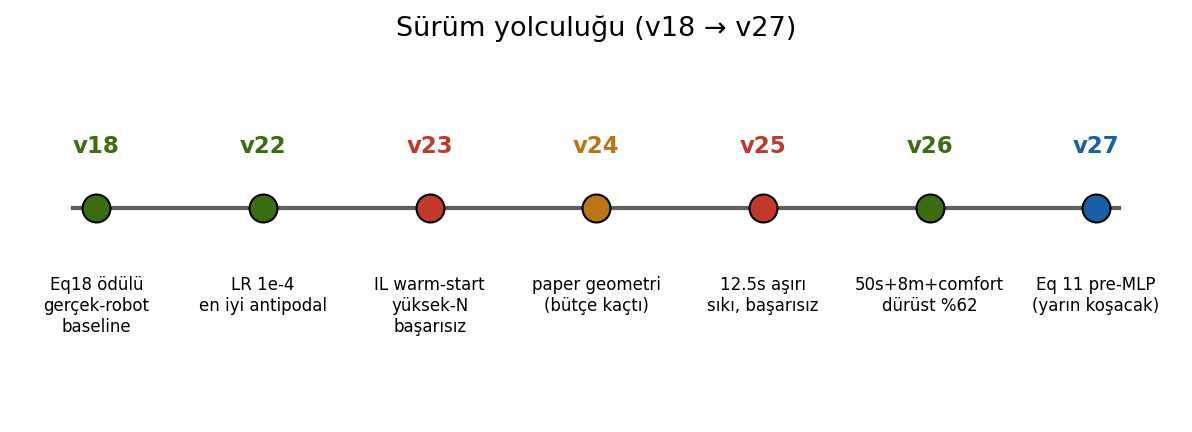
\includegraphics[width=0.96\textwidth]{figures/fig_journey.png}
\caption{v18'den v27'ye sürüm zaman çizelgesi. Yeşil: olumlu kilometre taşı; kırmızı: çürütülen
hipotez; turuncu: artefakt/kalibrasyon; mavi: planlanan deney.}
\label{fig:journey}
\end{figure}

\begin{table}[H]
\centering
\caption{Sürüm özeti ve çıkarımlar.}
\begin{tabular}{@{}llp{8.4cm}@{}}
\toprule
\textbf{Sürüm} & \textbf{Değişiklik} & \textbf{Sonuç / çıkarım} \\
\midrule
v18 & Eq 18 ödülü & 0.26 m/s gerçek-robot baseline; ilk geçen kapı. \\
v22 & LR $5\!\times\!10^{-5}\!\rightarrow\!10^{-4}$ & En iyi (zorlu) antipodal rejim sonucu; LR ana frendi. \\
v23 & IL (BC) ısıtması & Yüksek-N'de regresyon (N=10: 36$\rightarrow$22); hipotez çürütüldü. \\
v24 & Paper geometri & ``\%0 alarmı'' artefakttı (eğitim/değ.\ bütçe uyumsuzluğu). \\
v25 & Bütçe 12.5 s & Aşırı-sıkı (çarpışma-baskın \%62 tavanı); durduruldu. \\
v26 & 50 s + 8 m + konfor-norm. & \textbf{En iyi paper-rejim}; dürüst N=10 \%61.6; zaman aşımı 0. \\
v27 & + Eq 11 ön-MLP & Tek-değişkenli mimari sadakat denemesi (yarın). \\
\bottomrule
\end{tabular}
\label{tab:versions}
\end{table}

% ===================== 4. SONUÇLAR =====================
\section{Sonuçlar (v26)}

\subsection{Dürüst yoğunluk taraması}

v26'nın çok-tohumlu dürüst sonuçları Tablo~\ref{tab:density} ve Şekil~\ref{fig:density}'de verilmiştir.
\emph{Zaman aşımı her yoğunlukta \%0'dır}; bu, v26'nın temel tezini (50 s bütçe + 8 m geçiş + konfor
gradyanı) doğrular: robotun zaman açlığı tamamen ortadan kalkmıştır ve başarısızlık artık saf çarpışmadır.

\begin{table}[H]
\centering
\caption{v26 dürüst çok-tohumlu yoğunluk taraması (5 tohum $\times$ 50 bölüm = 250 bölüm/yoğunluk).}
\begin{tabular}{@{}ccccc@{}}
\toprule
\textbf{N (yaya)} & \textbf{Başarı} & \textbf{\%95 GA} & \textbf{Çarpışma} & \textbf{Zaman aşımı} \\
\midrule
5  & \%74.8 & [69.4,\ 80.2] & \%25.2 & \%0 \\
10 & \%61.6 & [55.6,\ 67.6] & \%38.4 & \%0 \\
15 & \%53.2 & [47.0,\ 59.4] & \%46.8 & \%0 \\
20 & \%43.6 & [37.5,\ 49.7] & \%56.4 & \%0 \\
\bottomrule
\end{tabular}
\label{tab:density}
\end{table}

\begin{figure}[H]
\centering
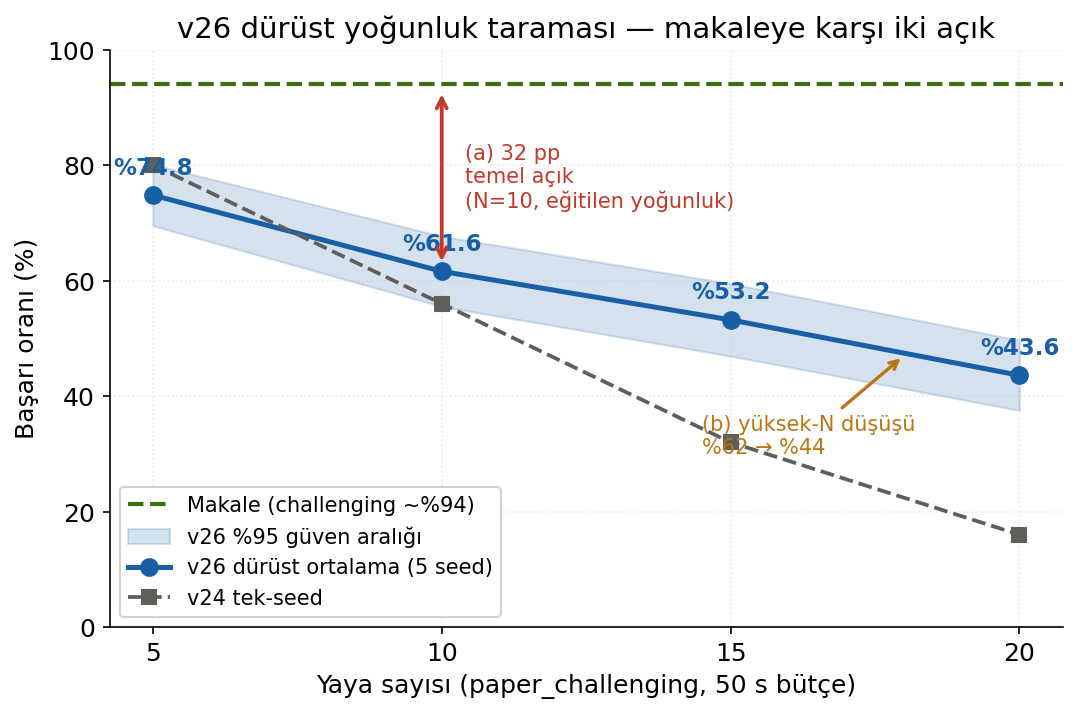
\includegraphics[width=0.82\textwidth]{figures/fig_density.png}
\caption{v26 dürüst yoğunluk eğrisi (mavi, \%95 GA bandı) ile makale hedefi (\%94, yeşil) ve eski
v24 tek-tohumlu tarama (gri) karşılaştırması. İki açık görünür: (a) N=10'da 32 puanlık temel açık,
(b) yüksek-N düşüşü.}
\label{fig:density}
\end{figure}

\subsection{Gerçek yörüngeler}

Şekil~\ref{fig:traj}, eğitilmiş politikanın kalabalık içinde ürettiği gerçek yörüngeleri gösterir.
Robot, düşük yoğunlukta kümeleri başarıyla dolaşır; yüksek yoğunlukta (N=20) güzergâh daralır ve
çarpışma olasılığı artar — bu, Tablo~\ref{tab:density}'deki sayısal düşüşle tutarlıdır.

\begin{figure}[H]
\centering
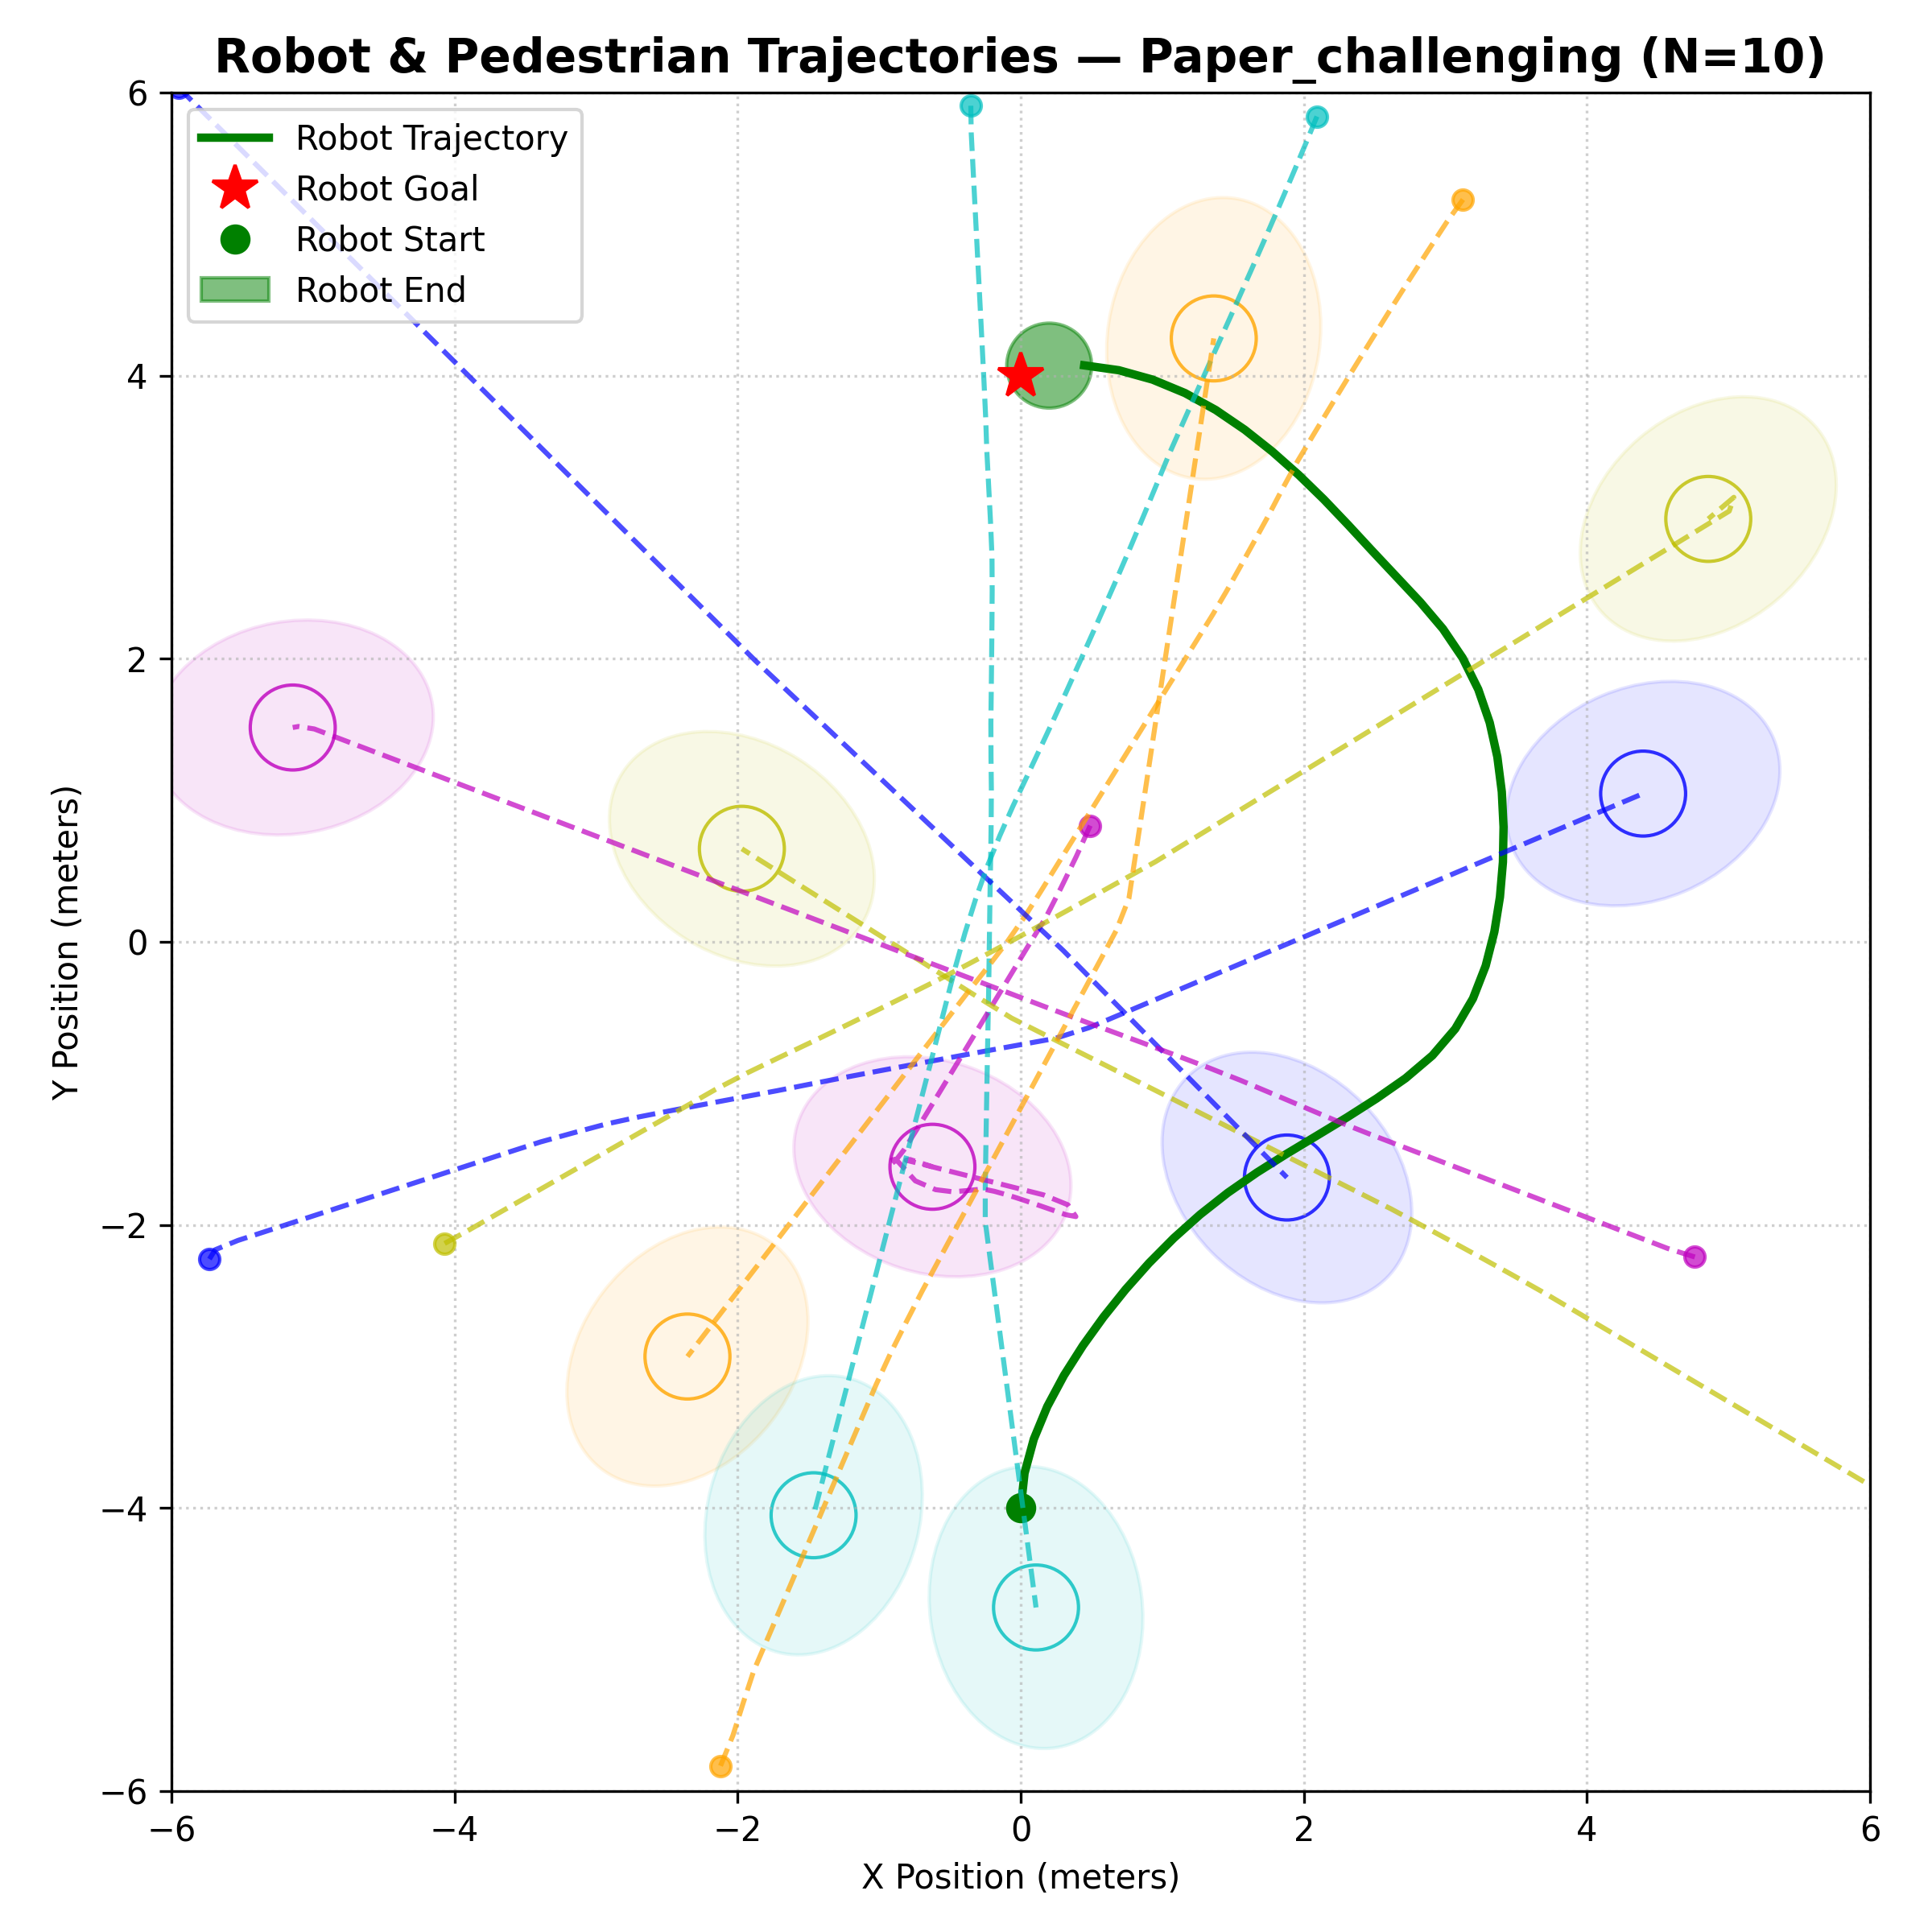
\includegraphics[width=0.48\textwidth]{figures/traj_n10.png}\hfill
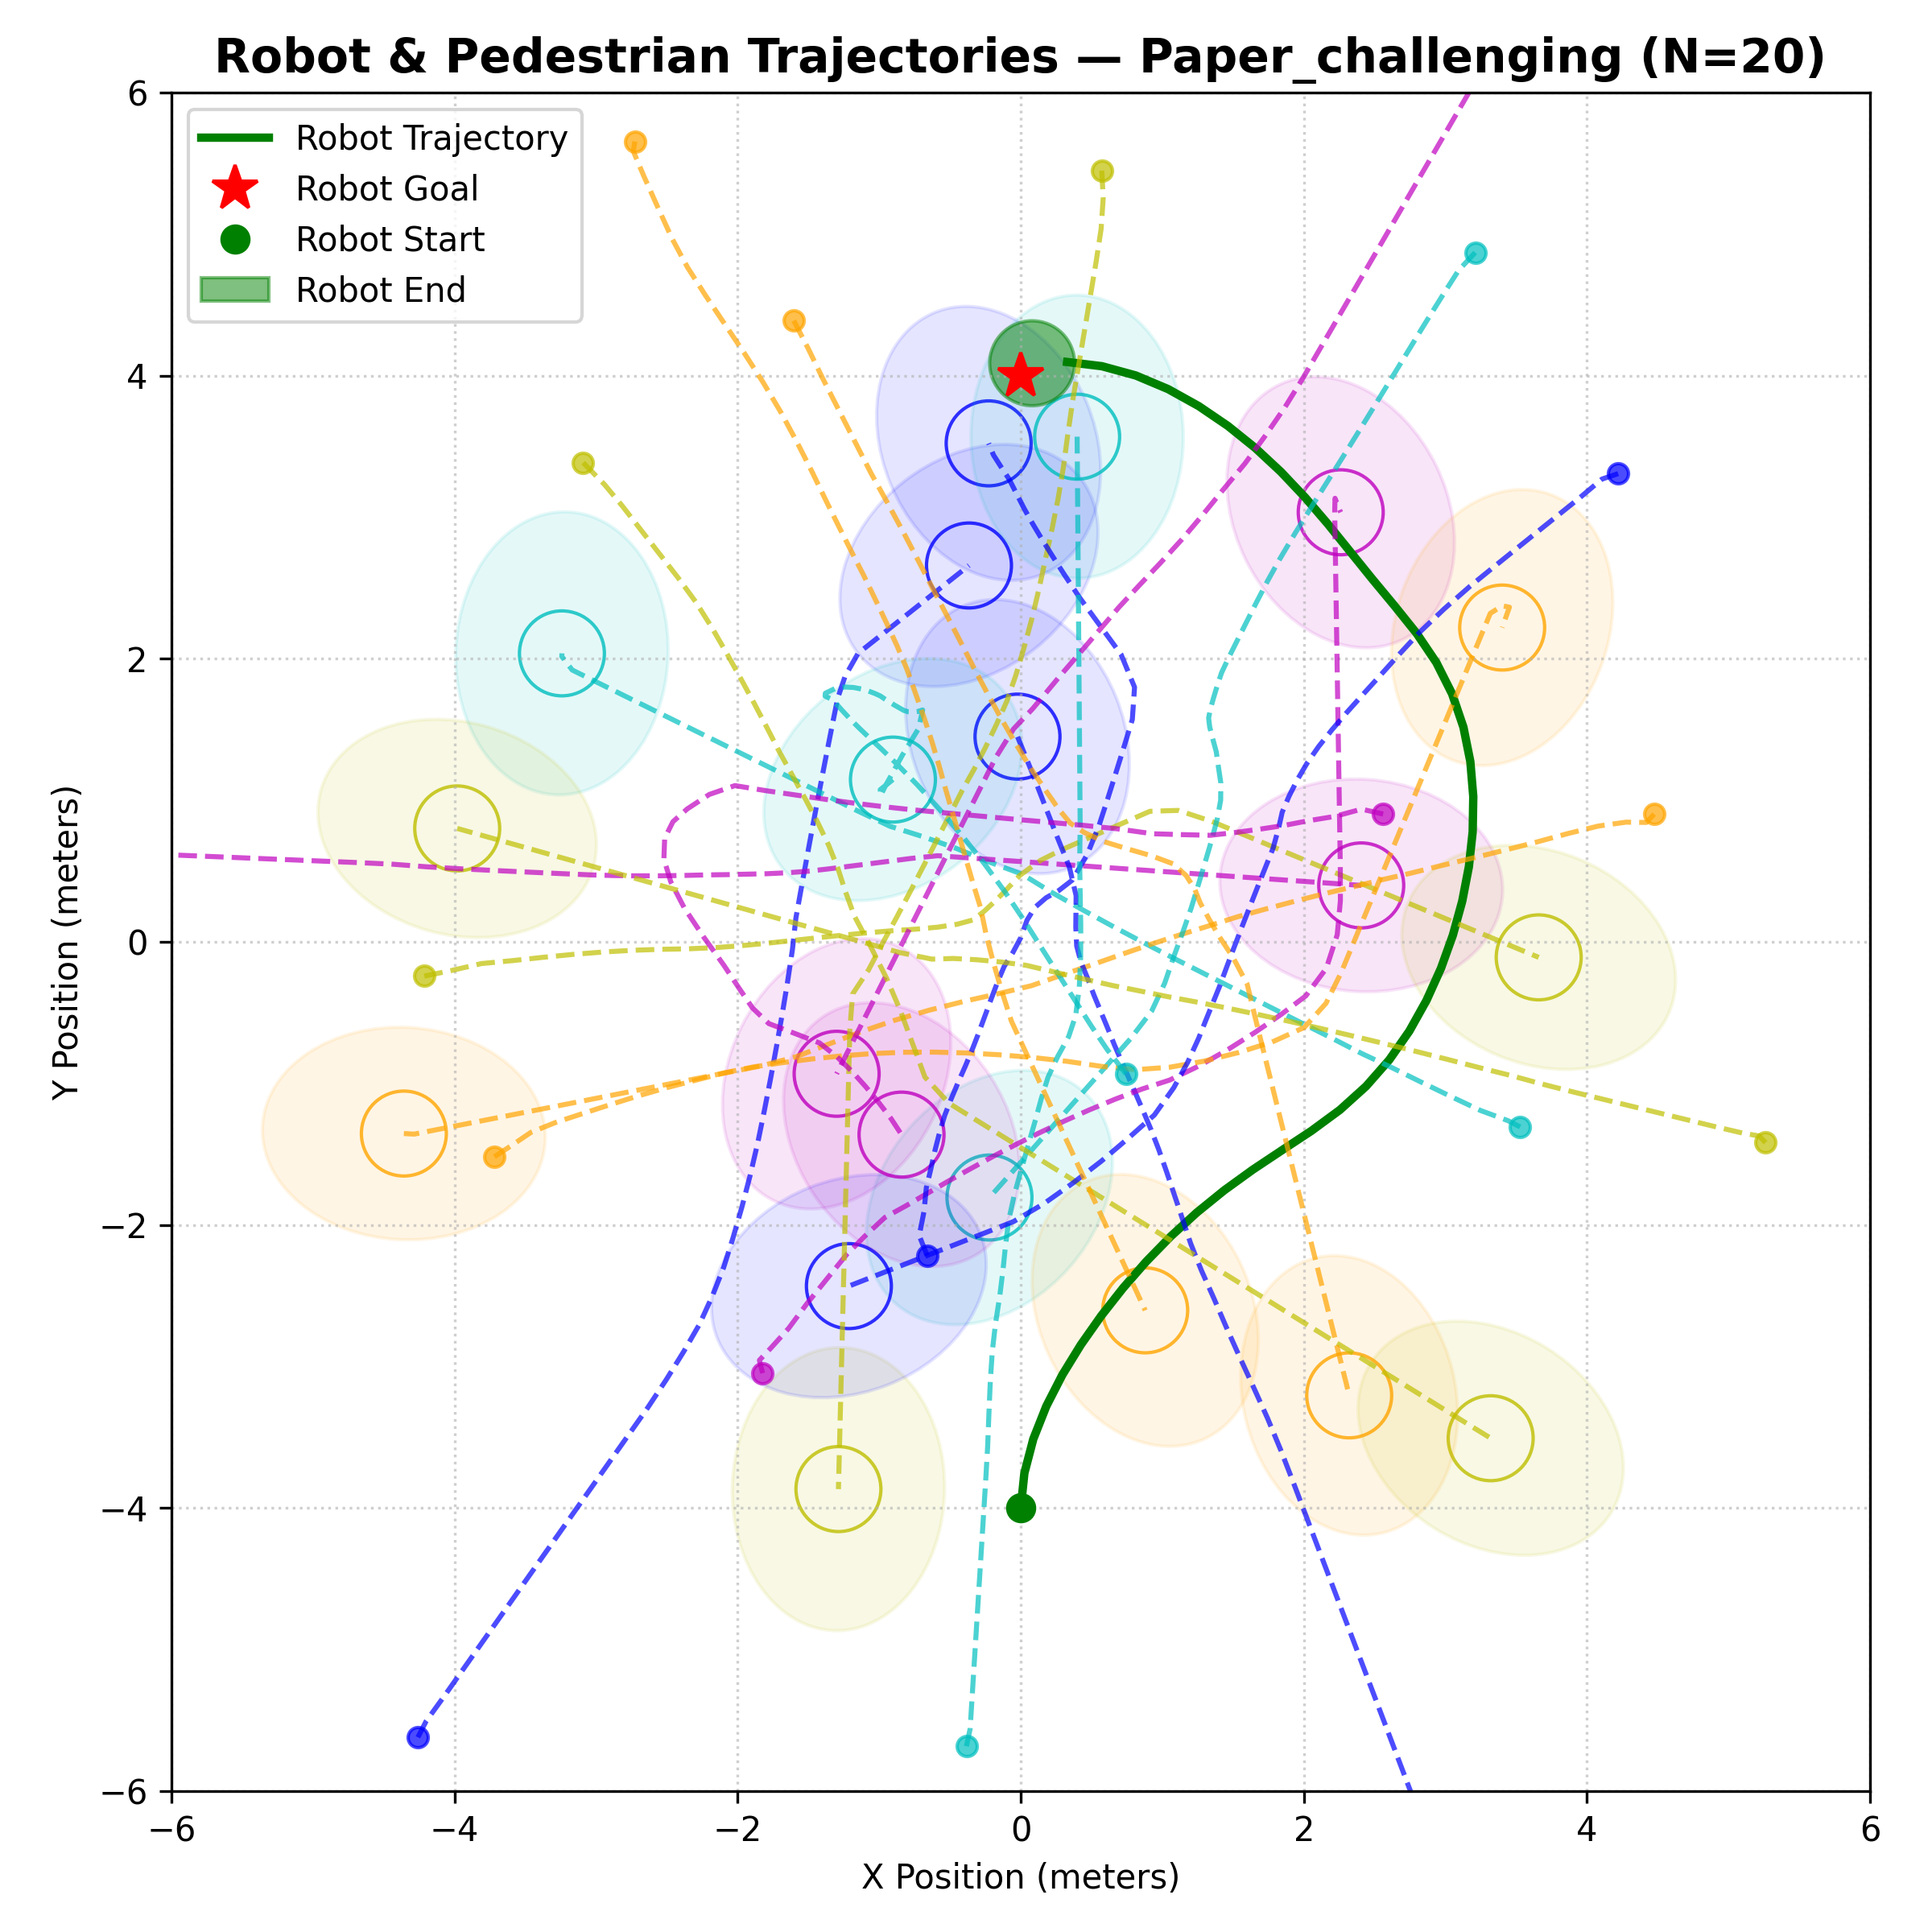
\includegraphics[width=0.48\textwidth]{figures/traj_n20.png}
\caption{Örnek yörüngeler: N=10 (sol) ve N=20 (sağ), \texttt{paper\_challenging}. Yoğunluk arttıkça
çarpışmasız güzergâh bulmak zorlaşır.}
\label{fig:traj}
\end{figure}

\subsection{Metodoloji bulgusu: ``best holdout'' seçim-saplıdır}

Bu projedeki en önemli metodolojik düzeltme burada ortaya çıktı. Eğitim sırasında ``best'' checkpoint,
holdout genelist-min ölçütü yeni bir maksimuma ulaştığında kaydedilir; ancak her holdout değerlendirmesi
\emph{farklı} bir tohum kümesi kullanır (\texttt{base\_seed = seed + 10000 + adım}). 2.5\,M boyunca
$\sim$58 gürültülü değerlendirme (her biri 50 bölüm, SE$\,\approx$7 puan) yapıldığından, bu serinin
\emph{maksimumu} yukarı yönlü saplıdır.

\begin{kritik}[Yerel kanıt — aynı checkpoint, sadece tohum farkı]
İndirilen \texttt{sncp\_ppo\_v26.pt} üzerinde, N=10 challenging için: \textbf{tohum 100} (sweep)
$\rightarrow$ \textbf{\%56}; \textbf{tohum 2{,}221{,}882} (en iyi adımın holdout tohumu)
$\rightarrow$ \textbf{\%76}. Aynı ağırlıklar, aynı yapılandırma — tek fark tohum. Yani rapor edilen
``best \%76'' gerçek bir kabiliyet değil, gürültünün şanslı tepesidir. Gerçek (önyargısız) değer
$\approx$\%61.6'dır (Şekil~\ref{fig:seedbias}).
\end{kritik}

\begin{figure}[H]
\centering
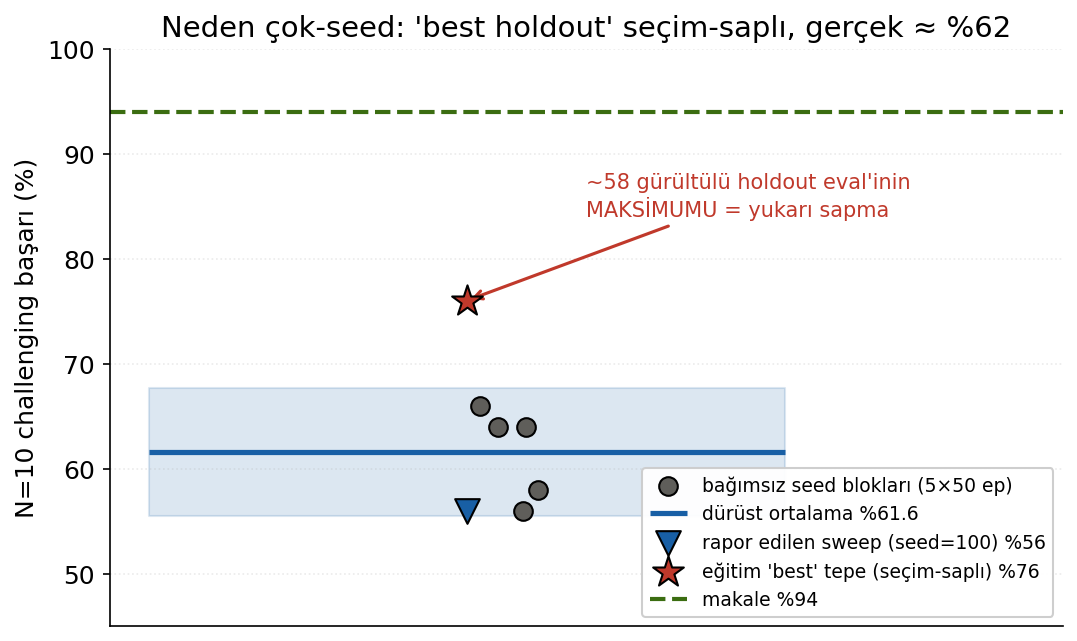
\includegraphics[width=0.78\textwidth]{figures/fig_seedbias.png}
\caption{N=10'da seçim sapması. Gri noktalar bağımsız tohum bloklarıdır; mavi bant dürüst ortalamanın
\%95 GA'sıdır. Kırmızı yıldız, eğitimin kaydettiği seçim-saplı ``best'' tepesidir (\%76); gerçek dağılım
ortalaması \%61.6'dır. Bu yüzden tüm sürüm kıyasları artık çok-tohumlu yapılır.}
\label{fig:seedbias}
\end{figure}

\subsection{Eğitim sağlığı}

Eğitim eğrisi (Şekil~\ref{fig:training}) sağlıklı bir tırmanış gösterir (generalist-min \%20$\rightarrow$\%76,
10 ``best'' olayı, çöküş yok); ardından final checkpoint best'in altına düşer (best$\rightarrow$final
degradasyonu). Değerlendirme \emph{best} checkpoint'i kullanır (kod: best yalnızca holdout-best'te kaydedilir;
final ayrı dosyaya gider), dolayısıyla yukarıdaki dürüst sayılar gerçek best ağırlıkları üzerindedir.

\begin{figure}[H]
\centering
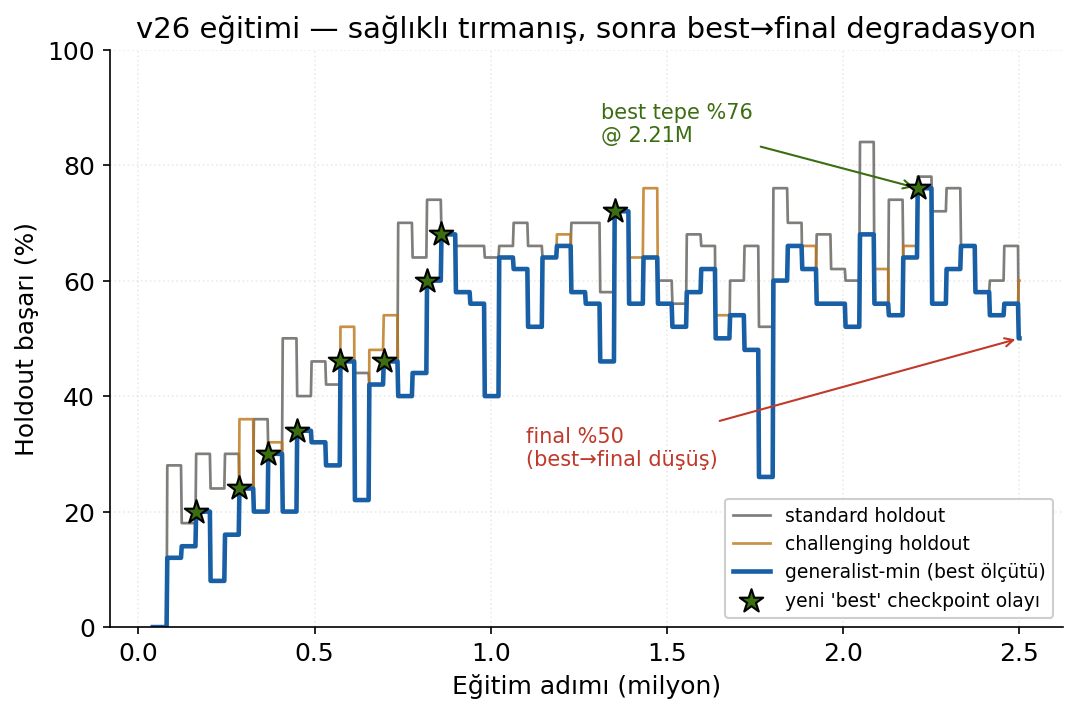
\includegraphics[width=0.78\textwidth]{figures/fig_training.png}
\caption{v26 eğitimi: standard/challenging holdout ve generalist-min eğrileri. Yeşil yıldızlar yeni
``best'' checkpoint olaylarıdır. Best tepe ($\approx$\%76 @ 2.21\,M) ile final arasındaki düşüş
(best$\rightarrow$final) görülmektedir; ancak Şekil~\ref{fig:seedbias} bu tepenin tohum-şansı olduğunu
gösterir.}
\label{fig:training}
\end{figure}

% ===================== 5. TARTIŞMA =====================
\section{Tartışma: Neden Henüz \%94 Değil?}

Dürüst sonuçlar, ``\%94'e neden ulaşmıyoruz?'' sorusunu iki ayrı ve daha keskin alt-soruya indirger.

\textbf{(a) Temel açık (N=10).} Eğittiğimiz yoğunlukta dahi \%61.6 ile \%94 arasında $\sim$32 puanlık fark
vardır. Bu, \emph{yoğunluk uyumsuzluğuyla açıklanamaz}; daha derin bir mimari/yöntem/sadakat farkına işaret
eder. En somut aday, makalenin Denklem~11 ön-MLP gömmesidir (aşağıda v27). Diğer adaylar: eylem dağılımı,
ORCA parametreleri, eval bölüm sayısı.

\textbf{(b) Yüksek-N düşüşü.} Başarı N=10'dan N=20'ye \%62$\rightarrow$\%44 düşer. Bunun bir kısmı eğitim/test
uyumsuzluğudur: biz sabit N=10'da eğitir, N=15/20'de test ederiz; makale ise 10--20 aralığında eğitir.
Bu açık için planlanan deney, eğitim yoğunluğunu $N\sim U(10,20)$ ile genişletmektir.

\begin{bulgu}[Hüküm]
v26, en iyi \emph{paper-rejim} sonucumuzdur (dürüst N=10 \%61.6) ve zaman aşımını tamamen kaldırmıştır.
v18 (0.26 m/s) gerçek-robot baseline'ı ayrı bir referans olarak kalır. Kalan açık iki bileşene ayrılmıştır;
ilk hedef \emph{temel} açıktır (a).
\end{bulgu}

% ===================== 6. SIRADAKİ ADIM: v27 =====================
\section{Sıradaki Deney: v27 (Denklem 11 Ön-MLP)}

Bir sonraki tek-değişkenli deney, makalenin Denklem~11 sıralamasını geri getirir: ham kenar girdisi
NCP'ye girmeden önce bir MLP ile gömülür,
\begin{equation}
\text{embedding}=\phi(\text{inputs},W_{\mathrm{mlp}}),\qquad
\text{feature},\,h'_{\mathrm{state}}=\psi(\text{embedding},h_{\mathrm{state}},W_{\mathrm{ncp}}). \tag{Eq.\ 11}
\end{equation}
Boyutlar makaleyle eşleşir (zaman kenarı 256, robot düğümü 128, dikkat 64; PDF s.\ 8). v26 varsayılanı bu
MLP'yi atlayıp ham 2/6 boyutlu sinyali doğrudan NCP'ye verir — Denklem~11'den gerçek bir sapma. v27, yalnızca
\texttt{-{}-pre\_mlp} bayrağını açar; başka \emph{hiçbir şey} değişmez (aynı tohum 42, 2.5\,M, rejim, bütçe,
geometri, konfor, $d_{\mathrm{col}}$).

\begin{yontem}[v27 değerlendirme planı]
Colab'da eğit (main'den çeker) $\rightarrow$ \texttt{sncp\_ppo\_v27.pt} indir $\rightarrow$ v26 ile
\emph{birebir aynı} protokolde yerel çok-tohumlu tarama (5 tohum $\times$ 50 bölüm) $\rightarrow$ v27
ile v26'nın \%95 GA'larını yoğunluk başına karşılaştır. \textbf{Karar kuralı:} v27'nin GA'sı v26'nınkini
(74.8/61.6/53.2/43.6) bir veya daha fazla yoğunlukta — özellikle N=10 — açıkça geçerse, ön-MLP yardımcıdır.
\end{yontem}

\begin{uyari}[İki dürüst uyarı]
\textbf{1. Kapasite karıştırıcısı:} ön-MLP büyük bir parametre artışı getirir; bir kazanç ``Eq 11 sıralaması''
mı yoksa ``salt kapasite'' mi olduğunu tam ayrıştıramayabiliriz (ancak bu, makalenin kendi mimarisinde de
vardır). \textbf{2. Önceki null:} ön-MLP daha önce \emph{yanlış} rejimde (v22 antipodal) denenmiş ve katkı
görülmemişti; v27 doğru paper rejiminde tekrar dener — garanti yoktur.
\end{uyari}

\begin{uyari}[Genel sınırlamalar]
Eski sürümlerin ``best holdout'' sayıları seçim-saplıdır (yalnızca çok-tohumlu sweep güvenilir). Eğitim
tek tohumla (42) yapılır; tam bir varyans tahmini için çoklu eğitim-tohumu gerekir. Makaledeki bazı
ayrıntılar (eval bölüm sayısı, ORCA parametreleri) tam doğrulanamamıştır.
\end{uyari}

% ===================== 7. SONUÇ =====================
\section{Sonuç}

Sistematik bir teşhis dizisi, makale açığını yöntemden çıkarıp iki somut ve test edilebilir bileşene
indirgemiştir. v26, paper rejimini sadık biçimde kurar, zaman aşımını sıfırlar ve dürüst N=10 başarısını
\%61.6 olarak ölçer. Kritik bir metodolojik düzeltme — ``best holdout''un seçim-saplı olduğu — gelecekteki
tüm kıyasları çok-tohumlu zorunlu kılar. Bir sonraki tek-değişkenli adım, mimari sadakati artıran Denklem~11
ön-MLP (v27) olup yarın eğitilecektir; ardından yüksek-N için yoğunluk müfredatı ($N\sim U(10,20)$) gelir.

\end{document}
